\section*{Appendix}

[add picture of the relu function]



\begin{figure}[h]
\centering
\caption{Distribution of Log Duration by Earnings Category}
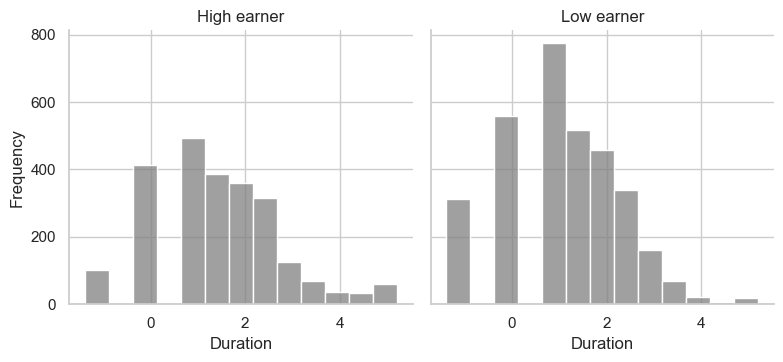
\includegraphics[width=\textwidth]{dist}
\label{fig:log_duration_distribution}
\end{figure}




\begin{table}[ht]
\centering
\caption{Comparison of Duration Across Injury Types Before and After 1980}
\label{tab:duration}
\begin{threeparttable}
\begin{tabular}{ccccccccc}
Injury Type & \textbf{1} & \textbf{2} & \textbf{3} & \textbf{4} & \textbf{5} & \textbf{6} & \textbf{7} & \textbf{8} \\
\hline
\hline
\addlinespace
after\_1980 = 0 & 778.25 & 282.00 & 1993.75 & 1663.25 & 5806.0 & 2649.75 & 194.25 & 413.5 \\
after\_1980 = 1 & 771.50 & 815.25 & 2341.75 & 1997.75 & 5362.5 & 2816.25 & 305.00 & 559.5 \\
Difference & -6.75 & 533.25 & 348.00 & 334.50 & -443.5 & 166.50 & 110.75 & 146.0 \\ \addlinespace
\end{tabular}
\begin{tablenotes}
\small
\item \textbf{Notes:}
\item \textbf{Injury Type}: Categories of injuries.
\item \textbf{after\_1980 = 0}: Duration of work leave before 1980.
\item \textbf{after\_1980 = 1}: Duration of work leave  after 1980.
\item \textbf{Difference}: Difference in duration values between after\_1980 = 1 and after\_1980 = 0.
\end{tablenotes}
\end{threeparttable}
\end{table}


% Please add the following required packages to your document preamble:
% \usepackage{graphicx}
\begin{table}[]
\centering
\caption{Regression Exclusion Test}
\label{tab:exclusion_test}
\resizebox{\columnwidth}{!}{%
\begin{tabular}{llllll}
Residual Degrees & Sum of Squared  & Degrees of  & Sum of Squares& F     & Pr(\textgreater{}(F)) \\
of Freedom                    &   Residuals                       &     Freedom Difference                          &         Difference                    &       &                       \\
\hline
\hline
\addlinespace
\addlinespace
2385.0           & 1.927912e+06             & 7.0                           & 32812.658                 & 5.798 & 0.000  \\ \addlinespace
\end{tabular}%
}
\begin{tablenotes}
    \small
    \item \textbf{Notes}:
    \item The table reports the results of the regression exclusion test. The test compares the full model with the restricted model, excluding the variable of interest.
    \small\item \textbf{Residual Degrees of Freedom}: Number of independent pieces of information remaining after fitting the model.
    \small\item \textbf{Sum of Squared Residuals}: Measure of the discrepancy between the observed data and the model's predictions, quantifying the variation not explained by the model.
    \small\item \textbf{Degrees of Freedom Difference}: Change in the degrees of freedom when moving from the restricted model to the full model.
    \small\item \textbf{Sum of Squares Difference}: Reduction in the sum of squared residuals when additional variables are added, indicating the improvement in model fit.
    \small\item \textbf{F}: F-statistic for the comparison of the two models.
    \small \item \textbf{Pr(>F)}: p-value for the F-test, indicating the significance of the difference between the models.
    \end{tablenotes}
\end{table}
